\begin{figure}[ht!]
    \centering
    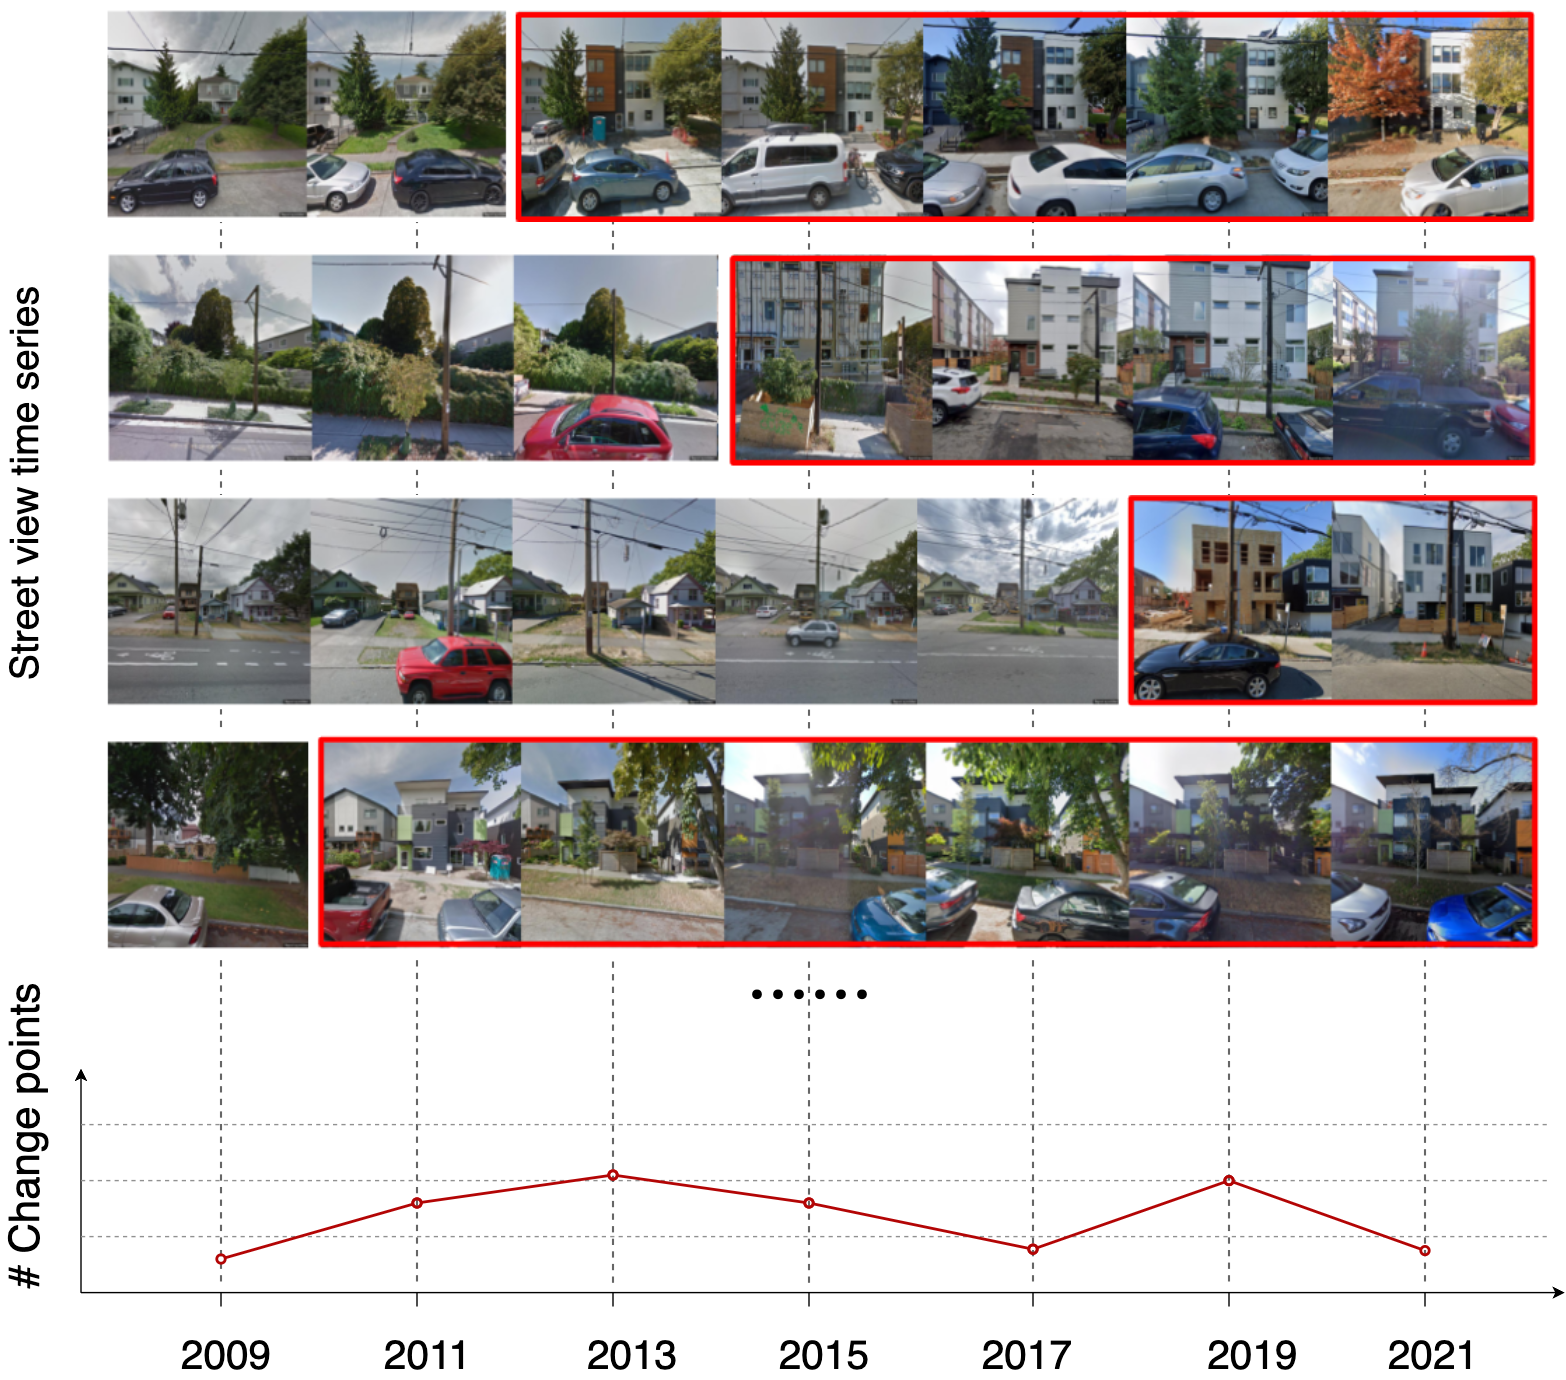
\includegraphics[width=1.0\linewidth]{figure/main.png}
    \caption{Detection of urban change points using street view time series. Red bounding boxes highlight transformations in the built environment at each location. By aggregating these detected change points within a neighborhood, we can evaluate the temporal dynamics of urban development.}
    \label{fig:main}
\end{figure}

% \begin{figure}[ht!]
%     \centering
%     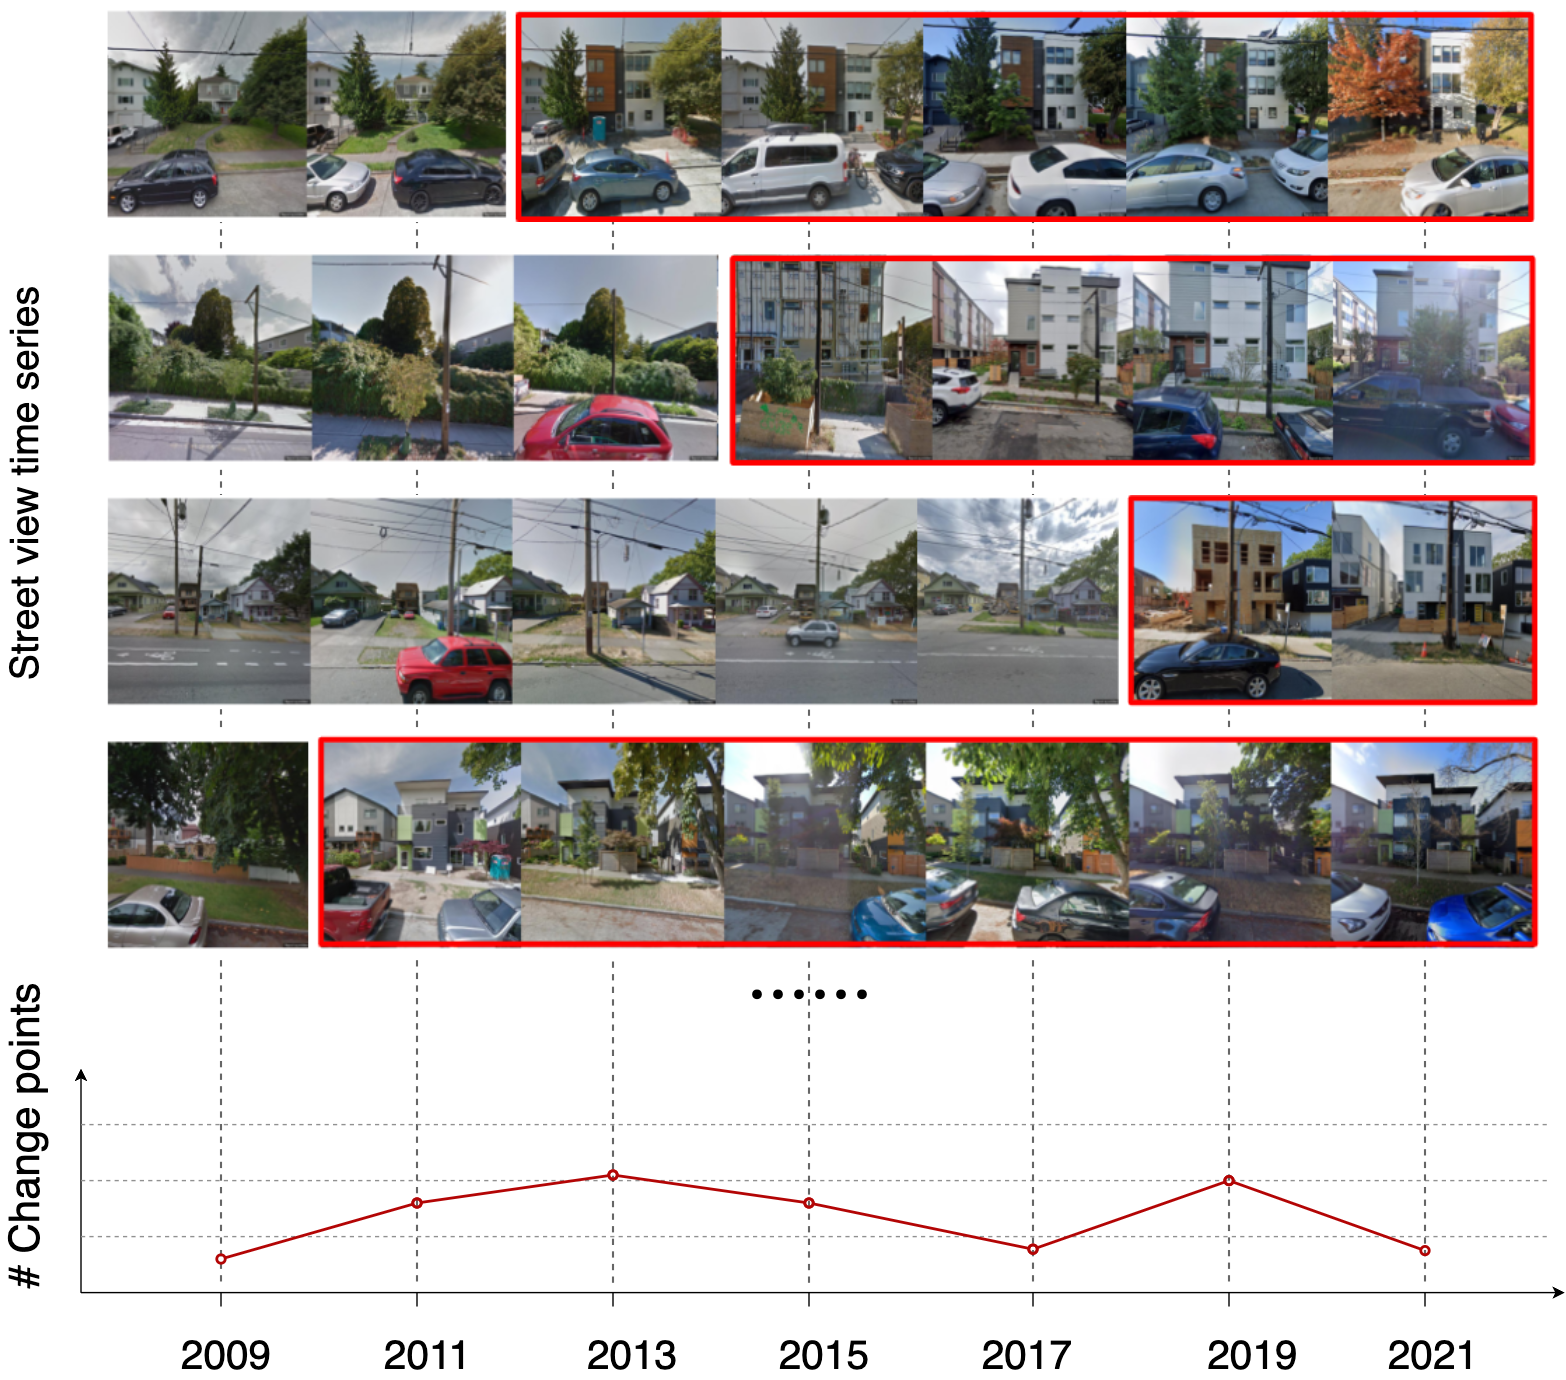
\includegraphics[width=1.0\linewidth]{figure/main.png}
%     \caption{Detecting urban change points from street view time series. Red bounding boxes denote the change of built environment in sampled coordinates. By aggregating the total number of change points inside the neighborhood, we could assess how cities change over time.}
%     \label{fig:main}
% \end{figure}